%*******************************************************************************
% Title:   Replicating Antman and Cortes (2023)
% Author:  Ibraheem Saqib Ellahi
% Build:   latexmk -pdf replication.tex   (run from paper/)
% Note:    No number is typed by hand. Every estimate arrives through \input of
%          an esttab fragment in ../output/tables, every figure through
%          \includegraphics from ../output/figures. Regenerate with: do run.do
%*******************************************************************************

\documentclass[11pt]{article}

\usepackage[margin=1in]{geometry}
\usepackage{booktabs}
\usepackage{graphicx}
\usepackage{amsmath}
\usepackage{float}
\usepackage{subcaption}
\usepackage{adjustbox}
\usepackage[round]{natbib}
\usepackage[hidelinks]{hyperref}

% Keep build timestamps out of the PDF metadata
\pdfinfoomitdate=1
\pdftrailerid{}

% esttab writes significance stars as \sym{...}; the fragments do not define it
\newcommand{\sym}[1]{\ifmmode^{#1}\else\(^{#1}\)\fi}

\graphicspath{{../output/figures/}}

% \input is not expandable, so inside a tabular it breaks the \bottomrule that
% follows it; the TeX primitive reads the fragment without that problem
\makeatletter
\newcommand{\tabinput}[1]{\@@input #1 }
\makeatother

% Derived numbers quoted in the text, e.g. \tOneDidYrsedPctBase (code/06_prose_numbers.do)
\IfFileExists{../output/tables/prose_numbers.tex}{% Generated by code/06_prose_numbers.do, do not edit by hand
\newcommand{\tOneDidYrsedPctBase}{7.6}  % Table 1 DiD years of ed as pct of 1931-35 HiSeg mean
\newcommand{\tOneDidJrhighPctBase}{18.8}  % Table 1 DiD jr high as pct of 1931-35 HiSeg mean
\newcommand{\tOneDidHschoolPctBase}{16.8}  % Table 1 DiD high school as pct of 1931-35 HiSeg mean
\newcommand{\tOneDidJrhighPp}{14.6}  % Table 1 DiD jr high in percentage points
\newcommand{\tOneDidHschoolPp}{8.0}  % Table 1 DiD high school in percentage points
\newcommand{\tTwoAYrsedPctBase}{9.0}  % Table 2A years of ed as pct of 1931-35 HiSeg mean
\newcommand{\tTwoAJrhighPctBase}{19.7}  % Table 2A jr high as pct of 1931-35 HiSeg mean
\newcommand{\tTwoAHschoolPctBase}{18.7}  % Table 2A high school as pct of 1931-35 HiSeg mean
\newcommand{\tTwoAJrhighPp}{15.3}  % Table 2A jr high in percentage points
\newcommand{\tTwoAHschoolPp}{9.0}  % Table 2A high school in percentage points
\newcommand{\pbLoSegN}{94}  % Panel B LoSeg people total
\newcommand{\pbLoSegPreN}{39}  % Panel B LoSeg born 1921-25
\newcommand{\pbLoSegPostN}{55}  % Panel B LoSeg born 1926-30
\newcommand{\pbHiSegN}{3,404}  % Panel B HiSeg people total
\newcommand{\pbLooMin}{\ensuremath{-}0.591}  % Panel B years of ed leave-one-out over LoSeg people min
\newcommand{\pbLooMax}{\ensuremath{-}0.228}  % Panel B years of ed leave-one-out over LoSeg people max
\newcommand{\pbLooMaxShift}{0.186}  % Panel B years of ed largest move from dropping one LoSeg person
}{}

\title{Replicating Antman and Cortes (2023):\\
The Long-Run Impacts of Mexican American School Desegregation}
\author{Ibraheem Saqib Ellahi\thanks{Code, data instructions, and outputs: \url{https://github.com/iellahi/Antman_Cortes_Repl}.}}
\date{Spring 2026}

\begin{document}

\maketitle

\begin{abstract}

\cite{antmancortes2023} examine long-run educational attainment for
Hispanics and non-Hispanic Whites in California after the 1947 \textit{Mendez v.\ Westminster} court decision ended de jure segregation of Mexican American schoolchildren. They use a difference-in-differences design across high and low segregation counties. In this document, I replicate Figure~\ref{fig:fig1}, Table~\ref{tab:table1}, Table~\ref{tab:table2} Panels A--C, and Figure~\ref{fig:fig2}. I extend Figure~\ref{fig:fig2} with event studies for the remaining two outcomes. Sample sizes are exact and point estimates differ only slightly, consistent with IPUMS revisions.

\end{abstract}

\section{Data and Empirical Strategy}
\label{sec:strategy}

\cite[p.~892]{antmancortes2023} use IPUMS 5 percent public use samples of the 1980, 1990, and 2000 US decennial censuses \citep{ipumsusa}. The sample consists only of people born in California. Years of schooling is built from IPUMS EDUCD. All estimates are unweighted, discussed in Section~\ref{sec:weights}.

Likely segregation is measured using Hispanic to non-Hispanic population ratios for all California counties in 1940. The difference-in-differences design compares HiSeg (counties above the seventy-fifth percentile) with LoSeg (counties below the twenty-fifth percentile) (p.~893). The treatment group is ages 2--6 (born 1941--45, $PostMendez_t=1$), and the comparison group is ages 12--16 (born 1931--35, $PostMendez_t=0$) in 1947. The 1936--1940 group is dropped because it would have been partially treated, similar to \cite{duflo2001} (p.~897). $HiSeg_c$ is the same for everyone in a county, so standard errors are clustered at the county level.

\begin{equation}
\label{eq:did}
Y_{ict} = \alpha + \pi \left( HiSeg_c \cdot PostMendez_t \right)
          + X_{ict}\,\beta + \mu_c + \delta_t + \varepsilon_{ict}
\end{equation}

Equation~\eqref{eq:did} is an OLS regression with two-way fixed effects (p.~896). $\pi$ is the difference-in-differences estimate. $Y_{ict}$ is the educational outcome of person $i$ in county $c$, born in year $t$. There are three outcomes: years of education, completing junior high, and completing high school. $X$ is a vector of controls. $\mu_c$ are county fixed effects and $\delta_t$ are birth-year fixed effects. $\varepsilon_{ict}$ is the error term.

\section[Results]{Results\protect\footnote{Figure and table titles in this section are reproduced verbatim from \citet{antmancortes2023}.}}
\label{sec:results}

\subsection{Educational attainment by cohort}
\label{sec:fig1}

Figure~\ref{fig:fig1} shows average years of education by birth cohort, plotted by age in 1947. The rise for HiSeg Hispanics is clear. It begins with cohorts aged ${\sim}$17 in 1947 and continues through cohorts still in school. This is consistent with desegregation raising schooling. The county gap for Whites is much smaller than Hispanics. The series converges for the youngest cohorts, the two White series meet and the Hispanic gap is at its smallest. The figure uses the same series, line styles, axis and legend as the published figure (p.~894).

\begin{figure}[H]
\centering
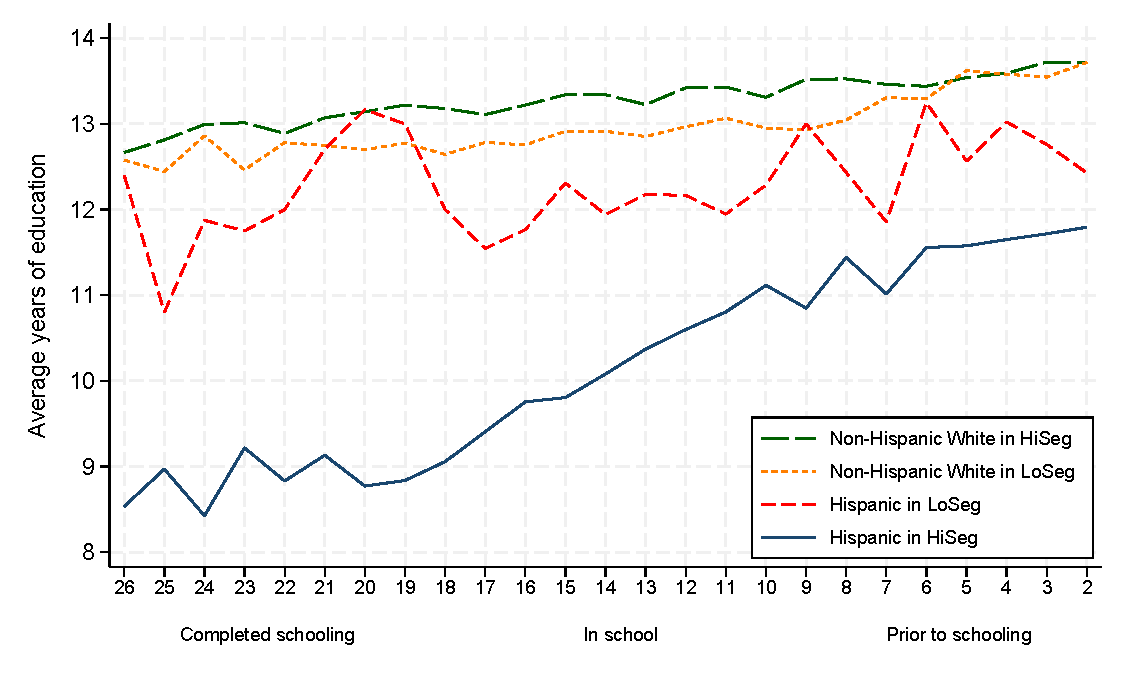
\includegraphics[width=\textwidth]{fig1_education_by_cohort.pdf}
\caption{Educational Attainment in High- and Low-Segregation Counties by Age at \textit{Mendez v.\ Westminster} School Desegregation Decision}
\label{fig:fig1}
\end{figure}

\subsection{Summary statistics and the raw difference-in-differences}
\label{sec:table1}

Table~\ref{tab:table1} shows mean outcomes by county group and cohort, the HiSeg--LoSeg gaps, and the raw difference-in-differences. All sample sizes and all junior high and high school values are identical to the published table (p.~896). There are small differences in years of education means, SDs, and the DiD in the second and third decimal. This is likely due to IPUMS revisions to education codes above 12 years. Binary outcomes cut at 8 and 12 years are unaffected.

\begin{table}[H]
\centering
\caption{Sample Descriptive Statistics on Mexican American Educational Attainment by Intent-to-Treat Status}
\label{tab:table1}
\begin{adjustbox}{max width=\textwidth}
\begin{tabular}{l*{7}{c}}
\toprule
\tabinput{../output/tables/table1_summary.tex}
\bottomrule
\end{tabular}
\end{adjustbox}
\end{table}

\subsection{Regression estimates}
\label{sec:table2}

Table~\ref{tab:table2a} shows the main estimates of equation~\eqref{eq:did}. Table~\ref{tab:table2b} shows the placebo test on cohorts born 1921--30 (too old to benefit); no estimate is positive. Table~\ref{tab:table2c} shows small negative estimates for non-Hispanic Whites. Minor differences from published estimates (p.~899, within one standard error) are likely driven by the years-of-education levels as well.

\begin{table}[!tbp]
\centering
\small
\caption{The Impact of \textit{Mendez v.\ Westminster} School Desegregation Decision on Educational Attainment}
\label{tab:table2}

\begin{subtable}{\textwidth}
\centering
\caption{Panel A. Hispanic Sample}
\label{tab:table2a}
\begin{tabular}{l*{3}{c}}
\toprule
\tabinput{../output/tables/table2_panelA.tex}
\bottomrule
\end{tabular}
\end{subtable}

\bigskip
\begin{subtable}{\textwidth}
\centering
\caption{Panel B. Placebo Sample (Hispanic Birth Cohorts 1921--1930)}
\label{tab:table2b}
\begin{tabular}{l*{3}{c}}
\toprule
\tabinput{../output/tables/table2_panelB.tex}
\bottomrule
\end{tabular}
\end{subtable}

\bigskip
\begin{subtable}{\textwidth}
\centering
\caption{Panel C. Non-Hispanic White Sample}
\label{tab:table2c}
\begin{tabular}{l*{3}{c}}
\toprule
\tabinput{../output/tables/table2_panelC.tex}
\bottomrule
\end{tabular}
\end{subtable}
\end{table}

\subsection{Event study}
\label{sec:fig2}

In Equation~\eqref{eq:es} below, a set of birth-year indicators replaces $PostMendez_t$. $\pi_\tau$ is the difference between HiSeg and LoSeg for cohort $\tau$. Figure~\ref{fig:fig2} shows negative estimates for cohorts aged 18--26 in 1947, estimates near zero for ages 12--17, and positive estimates for ages 2--11 (p.~900). The reference cohort is age 16 in 1947, marked by $\dagger$. Confidence intervals are wide because each cohort's LoSeg sample is small.

\begin{equation}
\label{eq:es}
Y_{ict} = \alpha + \sum_{\substack{\tau=1921 \\ \tau \neq 1931}}^{1945}
          \pi_\tau \left( HiSeg_c \cdot \mathbf{1}[t=\tau] \right)
          + X_{ict}\,\beta + \mu_c + \delta_t + \varepsilon_{ict}
\end{equation}

\begin{figure}[H]
\centering
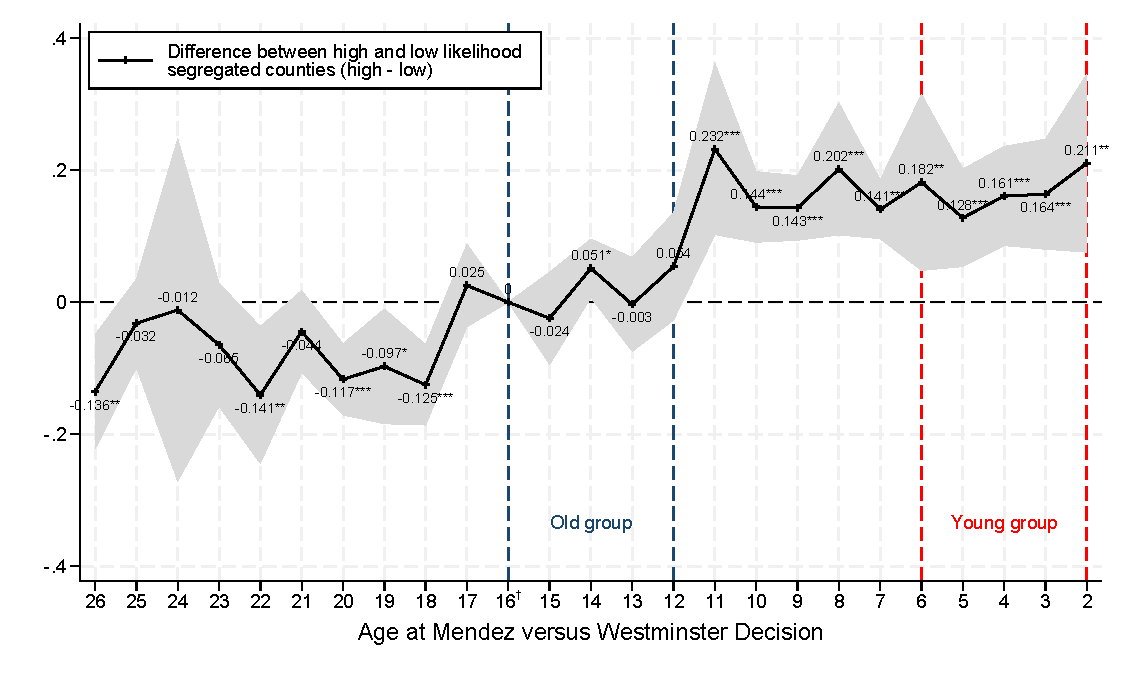
\includegraphics[width=\textwidth]{fig2_eventstudy_jrhigh.pdf}
\caption{Event Study Analysis—Educational Attainment for Hispanics, Junior High School Outcome}
\label{fig:fig2}
\end{figure}

\section{Discussion}
\label{sec:discussion}

\subsection{Threats to identification}
\label{sec:threats}

\paragraph{Parallel trends.} The design relies on the assumption that without the \textit{Mendez} decision, HiSeg and LoSeg areas would have moved together identically. A shock that threatens both cohorts differently is possible, even as fixed effects absorb county and cohort level shocks (e.g.,\ farm labor demand under the Bracero program (1942--64) concentrated in HiSeg Central Valley counties). Existing tests do support parallel trends. Table~\ref{tab:table2b} (placebo) has no positive estimates. In Figure~\ref{fig:fig2} (event study), ages 12--17 are near zero and show no drift before the treated cohorts. At the same time, however, these tests do not address migration.

\paragraph{Endogenous migration.} A county is the place people lived in 1980--2000 at ages 35--79. Families who moved after 1947 can affect the treatment variable. The direction of this selective sorting effect is ambiguous. It could be the case that educated Hispanics moved into HiSeg areas like Orange County to take advantage of the policy, pushing up the estimate. At the same time, educated Hispanics could have moved out of rural HiSeg areas, pushing it down. Childhood county-level data from the 1950 census linked to adult outcomes is one piece of data that could help. Ethnic attrition is another possibility, with some Hispanics no longer identifying as Hispanic \citep{duncantrejo2011}.

\subsection{A continuous-treatment alternative}
\label{sec:continuous}

An alternative could involve interacting a continuous 1940 Hispanic share (instead of the HiSeg\slash LoSeg) with $PostMendez_t$ using every identified county. 

\paragraph{Advantages.} The increased sample size allows for increased statistical power. There are no arbitrary percentile cutoffs. Estimates are then generalized across the entire distribution of counties, not just the extremes. Counties like Los Angeles and San Diego come back into the fold.

\paragraph{Disadvantages.} Such a model assumes linearity: a 1\% increase in Hispanic population share has a constant effect on segregation likelihood regardless of the baseline. Segregation likely follows a tipping point model. A certain critical mass of Hispanics is needed for a school district to invest in separate infrastructure. Middle counties excluded by the authors likely had fuzzy segregation practices, which means that they can add measurement error. Huge counties like Los Angeles and San Diego would dominate the estimate, though the paper does report that adding them to HiSeg changes little (p.~894, fn.~16). The authors' quartile approach likely maximizes the contrast between treated and untreated areas.

\subsection{Sampling weights}
\label{sec:weights}

The 1980 sample is self-weighting, every person a weight of 20. The 1990 and 2000 samples have varying weights (0--117 and 0--129) because long-form sampling rates differed by place size and responses were adjusted to population totals.

\paragraph{Point estimates.} Unweighted OLS estimates the average effect on a sampled person. If effects differ for different people, weighted and unweighted estimates may not represent the true average treatment effect for Hispanics \citep{solon2015}. If the impact of desegregation was heterogeneous (e.g.,\ different in rural areas than in urban ones), estimates would over or understate the aggregate benefit.

\paragraph{Standard errors.} Avoiding weights can maximize efficiency. Under the Gauss--Markov theorem, if the error terms are homoskedastic, unweighted OLS provides the best linear unbiased estimator (BLUE) with the lowest variance. Clustered standard errors already address heteroskedasticity. The small number of clusters presents a Type I error risk.

\section{Conclusion}
\label{sec:conclusion}

The replication succeeds: sample sizes are exact and estimates are within IPUMS revision noise. The event-study extension adds the same pattern for years of education and a weaker one for high school (Figures~\ref{fig:figA1} and~\ref{fig:figA2}). Section~\ref{sec:threats} points to limitations.

\appendix

% Appendix floats numbered A1, A2, ...
\setcounter{figure}{0}
\setcounter{table}{0}
\renewcommand{\thefigure}{A\arabic{figure}}
\renewcommand{\thetable}{A\arabic{table}}

\section{Additional event-study results}
\label{app:eventstudy}

Figure~\ref{fig:figA1} shows the event study for years of education. Figure~\ref{fig:figA2} shows it for high school completion. Table~\ref{tab:escoefs} lists every coefficient behind Figures~\ref{fig:fig2}, \ref{fig:figA1}, and~\ref{fig:figA2}.

\begin{figure}[H]
\centering
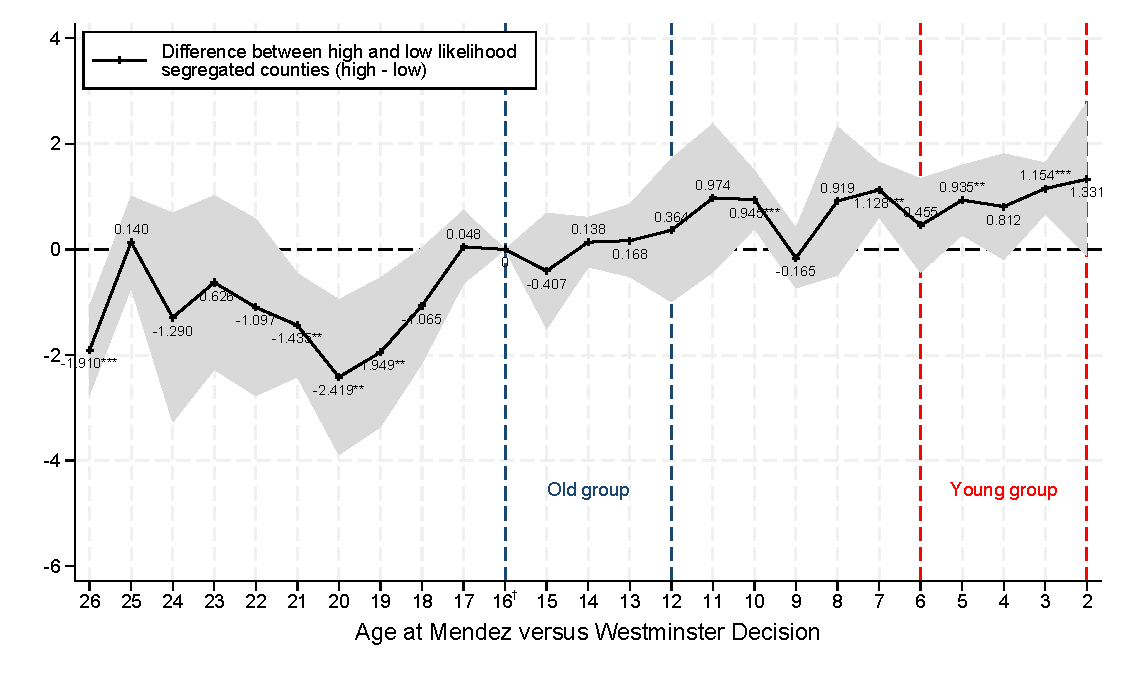
\includegraphics[width=\textwidth]{figA1_eventstudy_yrsed.pdf}
\caption{Event Study Analysis—Educational Attainment for Hispanics, Years of Education Outcome}
\label{fig:figA1}
\end{figure}

\begin{figure}[H]
\centering
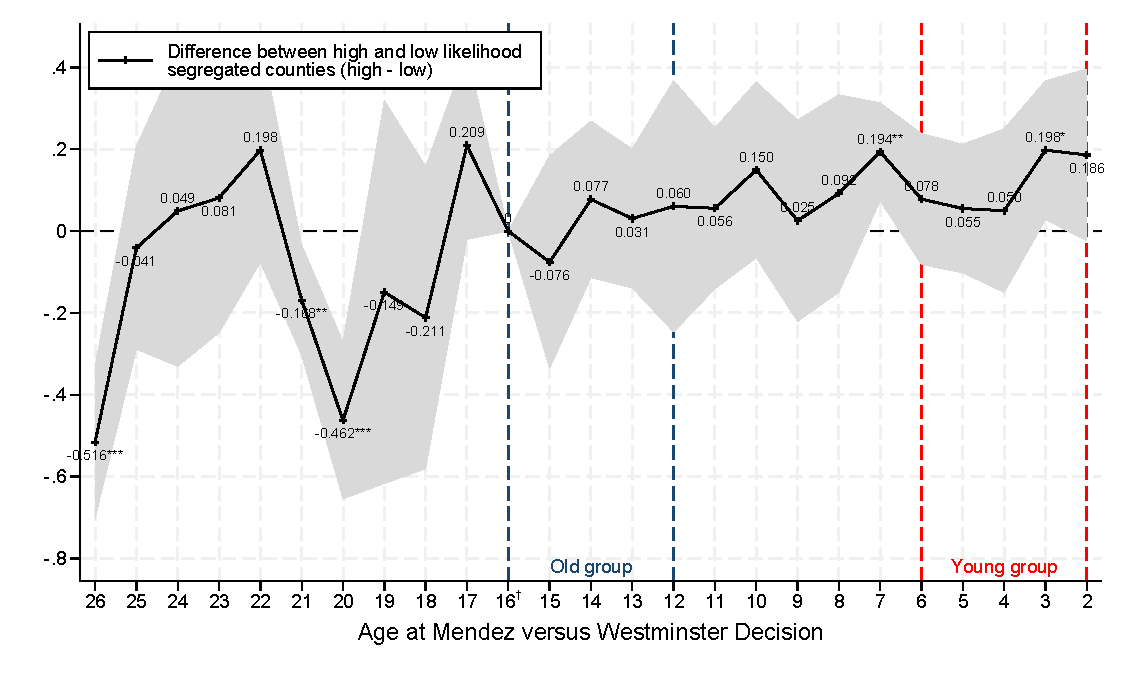
\includegraphics[width=\textwidth]{figA2_eventstudy_hschool.pdf}
\caption{Event Study Analysis—Educational Attainment for Hispanics, High School Outcome}
\label{fig:figA2}
\end{figure}

% Body rows, or a placeholder until the table has been generated
\IfFileExists{../output/tables/eventstudy_coefs.tex}
  {\newcommand{\esbody}{\tabinput{../output/tables/eventstudy_coefs.tex}}}
  {\newcommand{\esbody}{\multicolumn{8}{c}{[regenerates on the next run of \texttt{run.do}]}\\}}

\begin{table}[H]
\centering
\caption{Event Study Coefficients by Birth Cohort, All Three Outcomes}
\label{tab:escoefs}
\small
\begin{tabular}{cc*{6}{c}}
\toprule
& & \multicolumn{2}{c}{Jr.\ high (8+)} & \multicolumn{2}{c}{Years of education}
  & \multicolumn{2}{c}{High school (12+)} \\
\cmidrule(lr){3-4}\cmidrule(lr){5-6}\cmidrule(lr){7-8}
Age in 1947 & Birth year & Coef. & SE & Coef. & SE & Coef. & SE \\
\midrule
\esbody
\bottomrule
\end{tabular}
\begin{minipage}{\textwidth}
\footnotesize
\textit{Notes:} Coefficients $\pi_\tau$ from Equation~\eqref{eq:es}, one regression per outcome, same sample as Figure~\ref{fig:fig2}. Standard errors clustered by county. The 1931 cohort (age 16 in 1947) is the reference and is set to zero. *** $p<0.01$, ** $p<0.05$, * $p<0.10$.
\end{minipage}
\end{table}

\section{Reproducibility}
\label{app:repro}

\begin{itemize}
  \item The IPUMS extract is not redistributable; see README.
  \item One command regenerates every number and figure: \texttt{cd} to the repo root, \texttt{do run.do}
  \item \texttt{estout} is vendored in \texttt{code/ado/estout} so no package installation is needed
  \item folder map below
\end{itemize}

\begin{small}\begin{verbatim}
run.do                    master; sets paths, runs code/01-06 in order
code/01_build_data.do     IPUMS extract  -> data/clean/antman_cortes_clean.dta
code/02_figure1.do        cohort means   -> output/figures/fig1_*
code/03_table1.do         Table 1        -> output/tables/table1_summary.*
code/04_table2.do         Table 2 A/B/C  -> output/tables/table2_panel*.*
code/05_event_study.do    Figures 2/A1/A2, output/tables/eventstudy_coefs.*
code/06_prose_numbers.do  numbers cited in the text -> output/tables/prose_numbers.*
code/lib/yrsed.do         EDUCD -> years of schooling crosswalk
\end{verbatim}\end{small}

\bibliographystyle{plainnat}
\bibliography{references}

\end{document}
